% First split after inserting c: create node 3 for bb and node 4 for bbc.
% The remaining suffixes bc and c are inserted in the next diagram.
% Regenerate from this directory:
% latex -interaction=nonstopmode -halt-on-error suffix-tree6.tex
% dvisvgm --no-fonts --exact --bbox=papersize -o suffix-tree6.svg suffix-tree6.dvi
\documentclass[tikz,border=8pt]{standalone}
\usepackage{lmodern}
\usetikzlibrary{arrows.meta}
\definecolor{nodecolor}{HTML}{242A31}
\begin{document}
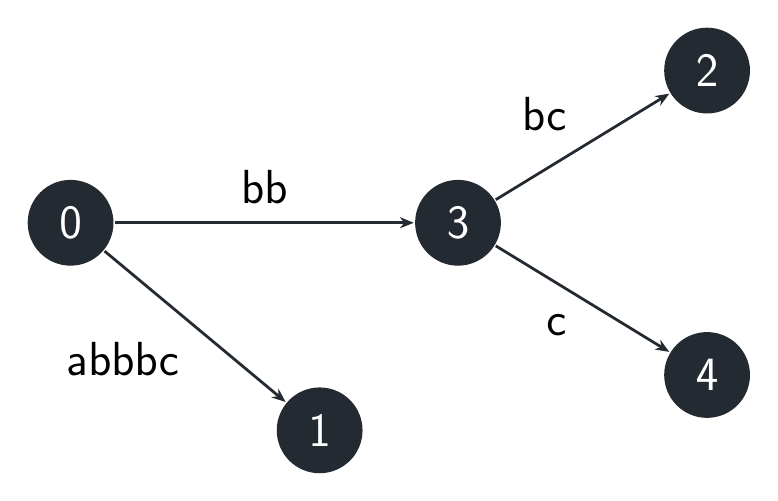
\begin{tikzpicture}[
  x=1pt,y=-1pt,line width=1pt,draw=nodecolor,
  font=\sffamily\fontsize{18}{21}\selectfont,
  vertex/.style={circle,fill=nodecolor,text=white,minimum size=31pt,inner sep=0pt},
  every edge/.style={draw,-{Stealth[length=5pt,width=4pt]}}
]
  \node[vertex] (n0) at (0,0) {0};
  \node[vertex] (n1) at (90,75) {1};
  \node[vertex] (n2) at (230,-55) {2};
  \node[vertex] (n3) at (140,0) {3};
  \node[vertex] (n4) at (230,55) {4};
  \path
    (n0) edge node[below left=2pt] {abbbc} (n1)
    (n0) edge node[above=3pt] {bb} (n3)
    (n3) edge node[above left=2pt] {bc} (n2)
    (n3) edge node[below left=2pt] {c} (n4);
\end{tikzpicture}
\end{document}
